\chapter{Technical Coordination and Management at Facilities}
\label{vl:tc-facility_mgmt}

[Bill]

This needs to include how we manage teams from consortia
e.g. students, equipment, etc. We need to say what is provided by TC,
e.g. techs, engineers, tools, etc.
\begin{enumerate}
 \item Technical coordination of activities {surf}: This section
   includes what TC provides and how it interfaces with consortia work
   at {surf}.
 \item Technical coordination of activities ITF: This section includes
   what TC provides and how it interfaces with consortia work at ITF.
 \item Technical coordination of activities at Ash River installation
   test site: This section includes what TC provides and how it
   interfaces with consortia work at Ash River (Should this go into
   APA? Or into Single Phase Installation and Integration?)
\end{enumerate}



There are two management teams responsibility for coordinating the
detector installation and integration for underground and at the
surface. The group responsible for activities in the underground areas
is referred to as the underground installation team (UIT).  On the
surface the surface installation team (SIT) coordinates the Logistics
Center where all DUNE shipping and receiving is initiated and the
Integration and Testing Facility (ITF) where the integration of the
APAs happen.  These installation teams include management, safety
officer, riggers and equipment operators needed to move all detector
components on the surface and underground. {surf} and the {cmgc} are
responsible for moving them from the headframe to the detector hall.

These two teams must work closely with the LBNF Logistics team at
{surf}, {cmgc}, the different consortia and technical coordination to
ensure that all components required for the infrastructure and
detectors are delivered in an organized and scheduled manner. During
Civil Construction the shaft is controlled by the {cmgc} and all loads
underground are managed by them.  The Logistics Center and ITF are
needed approximately 2 years before Beneficial occupancy of the North
Cavern.  During this time period it needs to develop a buffer of APAs
and begin the installation of the infrastructure underground. This
ramp-up of manpower helps develop a trained and organized team on the
surface that merges with the team underground.


\section{Surface Facilities}

Since no materials or equipment can be directly shipped to the Ross or
Yates headframe the Logistics Center is used for both short and
long-term storage and re-packaging before it is shipped underground.
The function of the Logistics Center is shown in
Figure~\ref{fig:orgchart_lc}.
\begin{dunefigure}[Logistics concept.]{fig:orgchart_lc}
  {Org Chart for the Logistics Center.}
  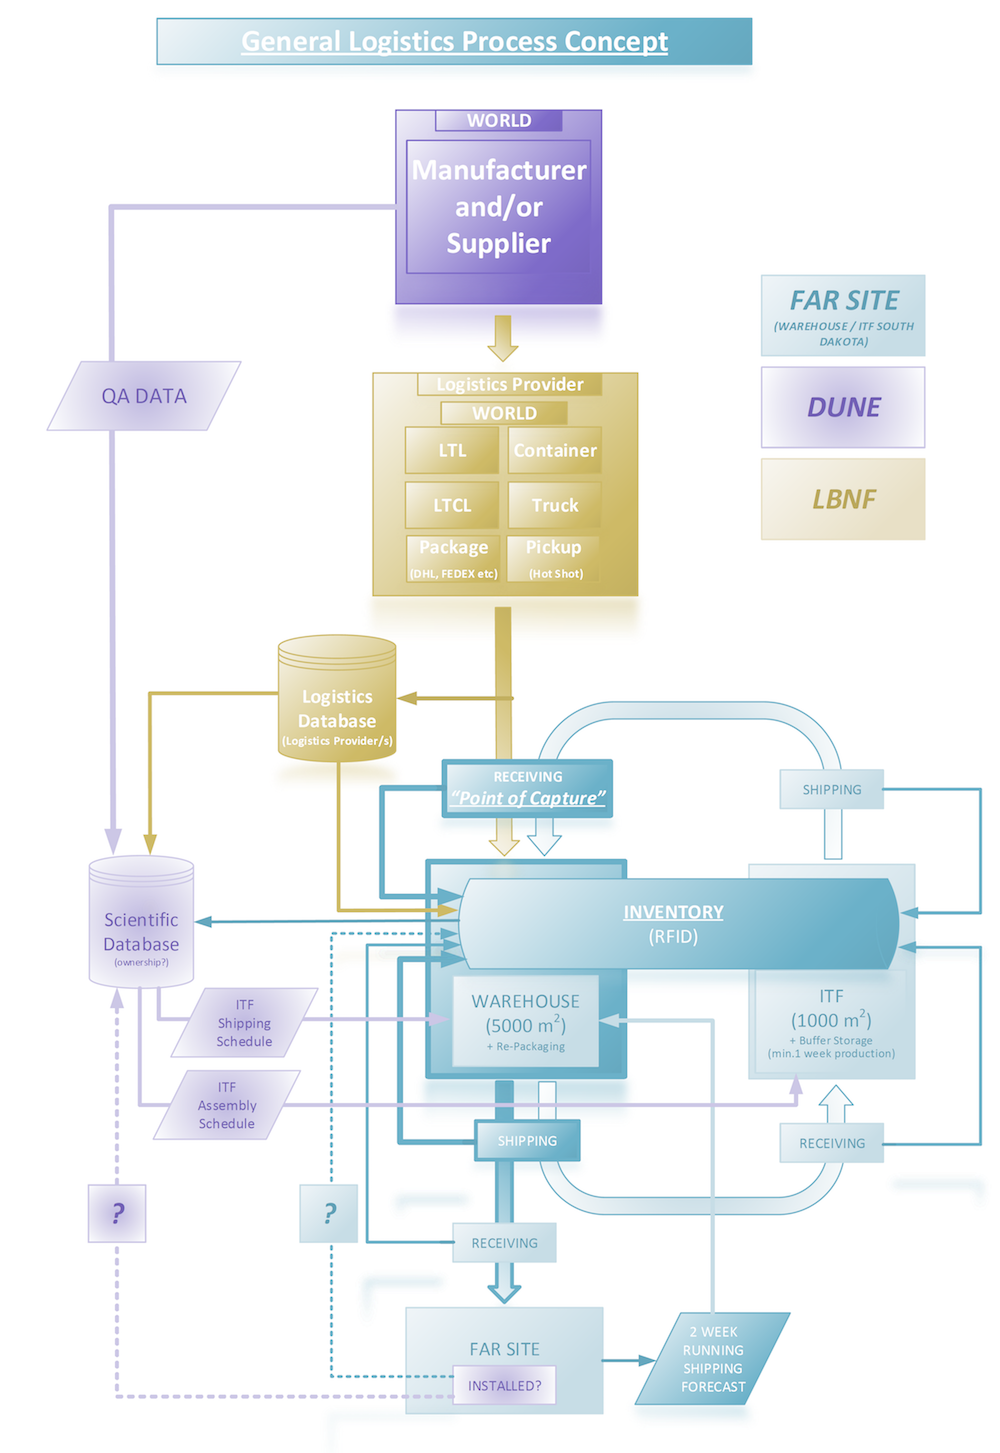
\includegraphics[width=0.85\textwidth]{logistics.png}
\end{dunefigure}
The Logistics center is also where everything is inventoried and
entered into the hardware data base.  The Logistics Center is also
responsible for trucking between the ITF and {surf} and dunnage coming
back.  TPC components that need to go to the Integration and Testing
Facility arrive at the Logistic Center are logged into the inventory
system them transported to the ITF as needed. Once the integration is
completed APA pairs are transported back to the Logistics Center ready
for shipment underground.  The team of riggers and equipment operators
are trained professionals that move all the TPC components and
infrastructure but also trained to assist when needed with the
integration. The organization of the Logistics Center and Integration
and Testing Facility are shown in Figure~\ref{fig:orgchart_itf}.
\begin{dunefigure}[Org Chart for the Logistics Center and Integration and Testing Facility.]{fig:orgchart_itf}
  {Org Chart for the Logistics Center and Integration and Testing
    Facility.}  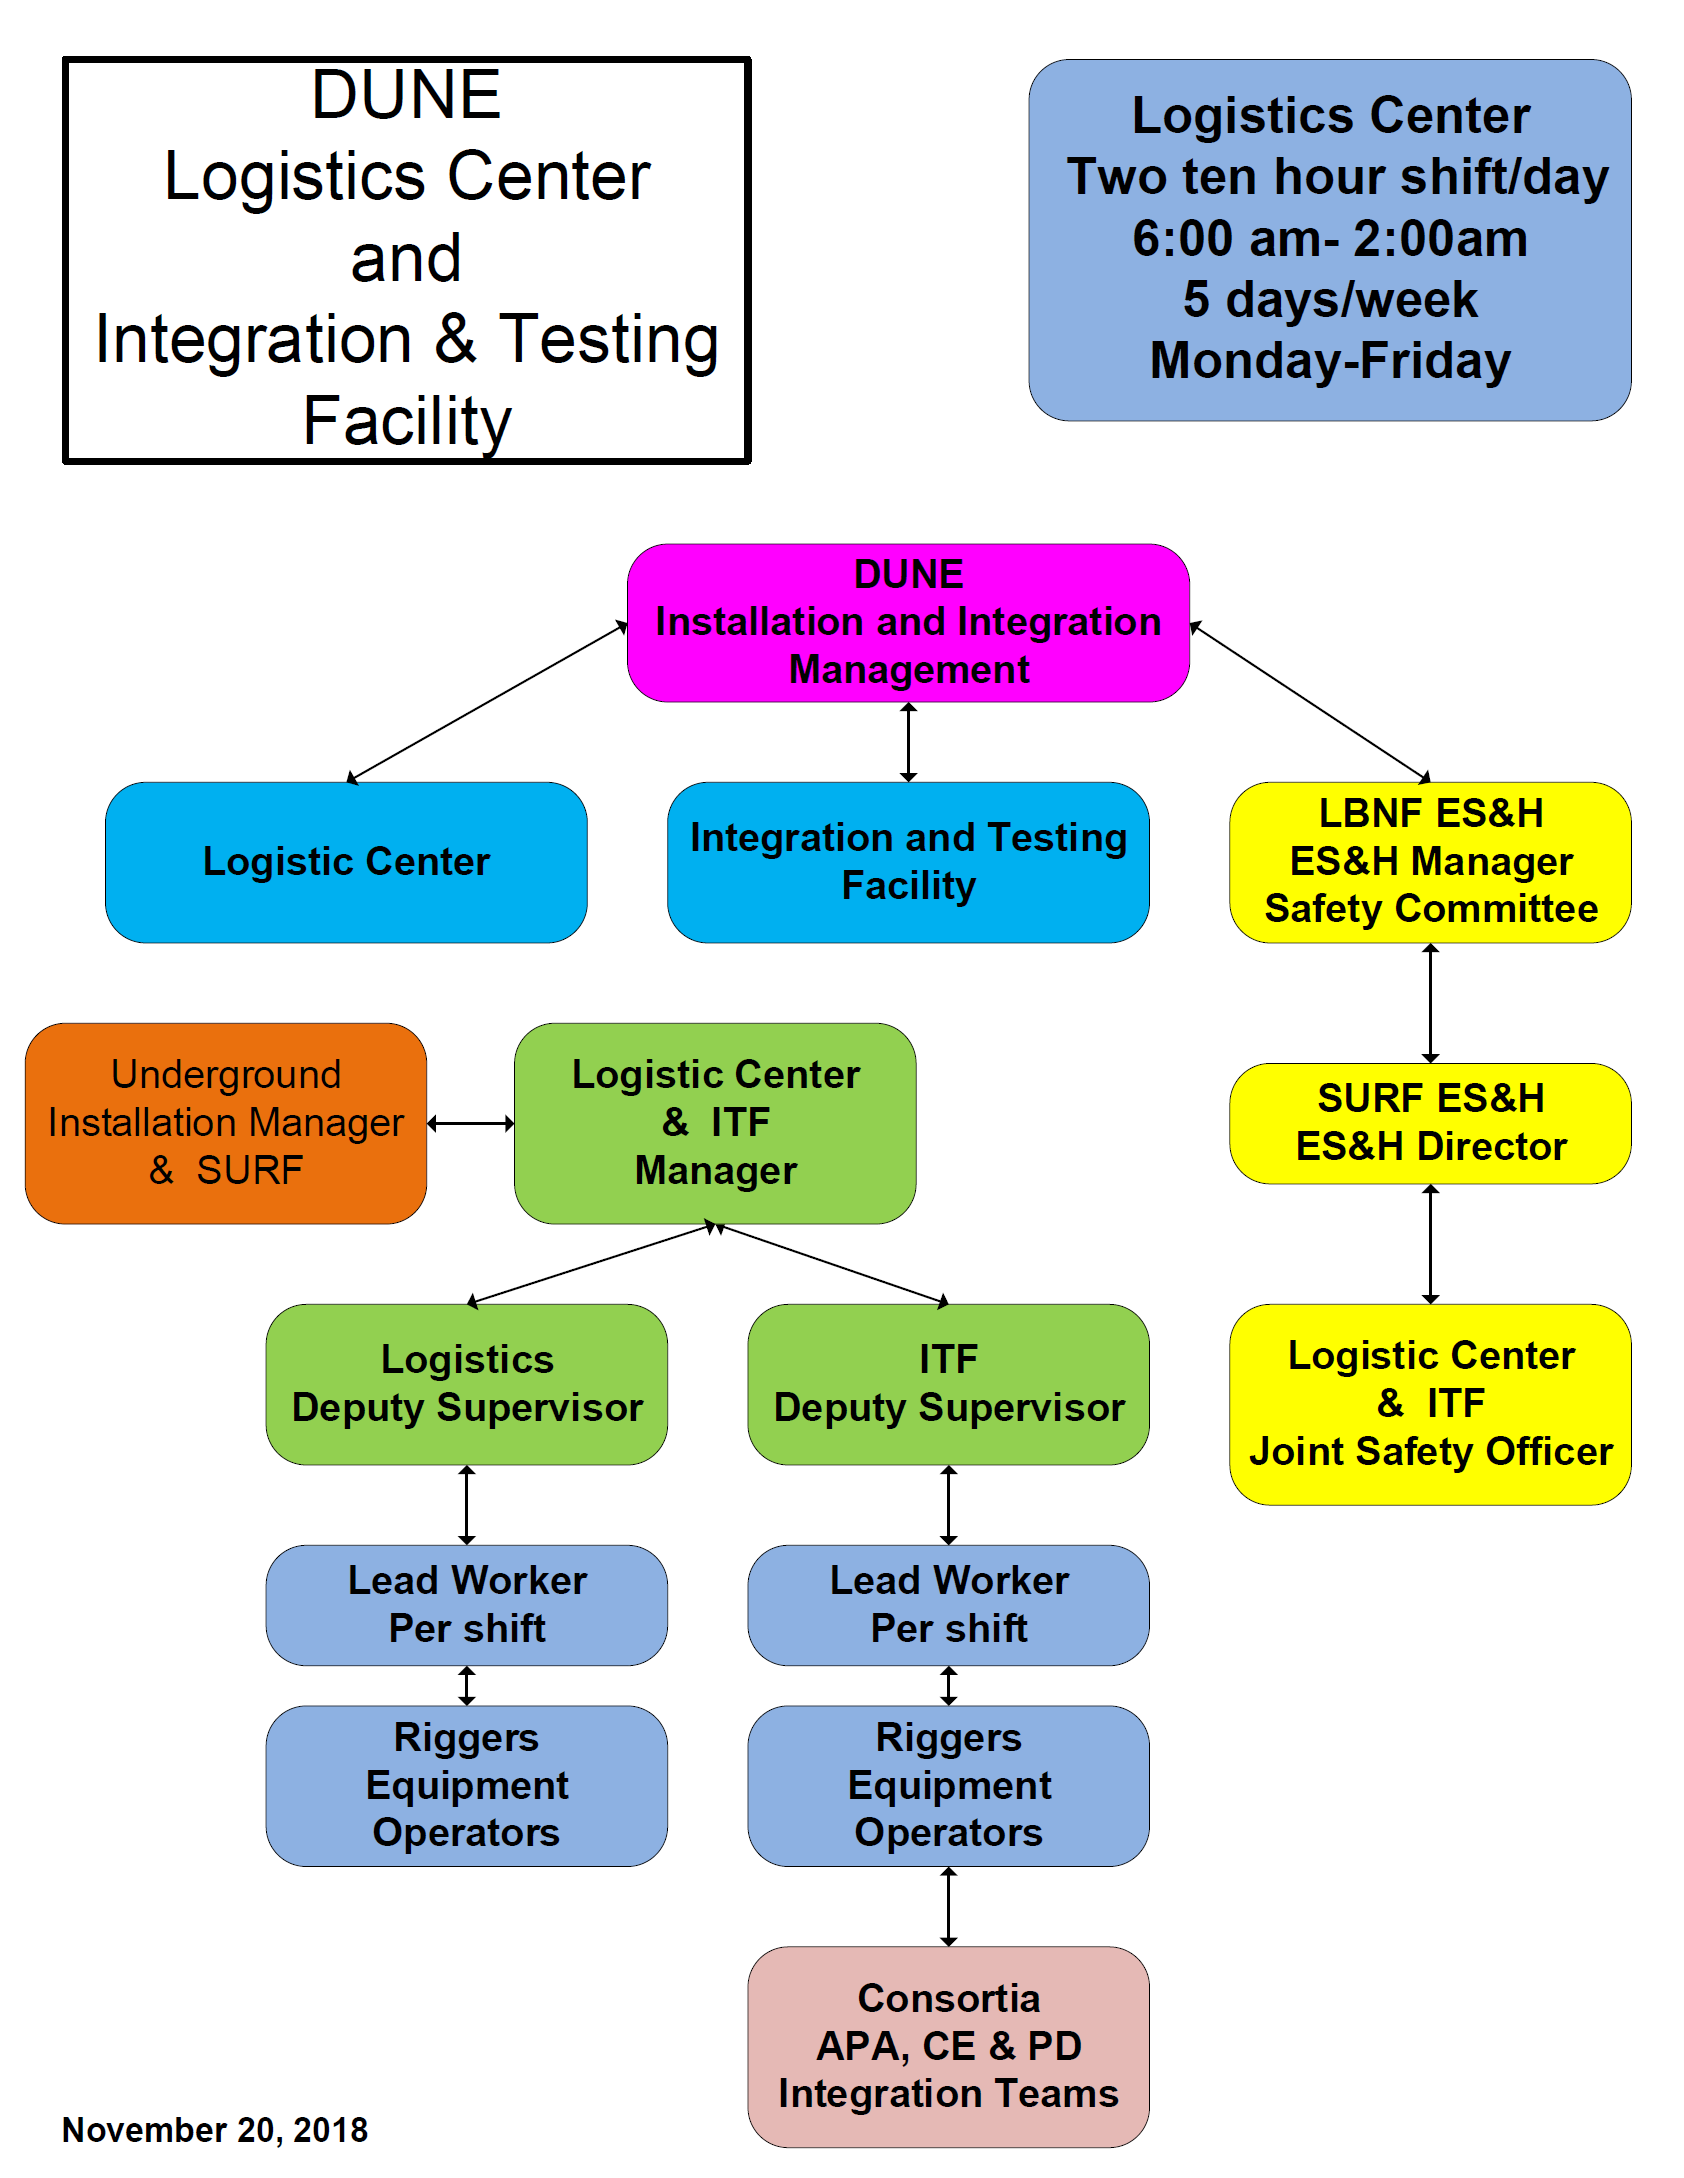
\includegraphics[width=0.85\textwidth]{lc.png}
\end{dunefigure}

\subsection{Logistics Center}

The Logistics Center is a shipping and handling facility, it has a
smaller crew than ITF, but it must operate 20 hours/day 5 days a week.
It will require 2 rigging/operator crews which will be managed by a
joint management team working in concert with the ITF.  There would be
a Manager and two deputy supervisors (Logistics Center and ITF),
administrative assistant and a safety officer working under the direction
of Fermilab Safety.  There would be a lead worker for each shift which
would direct the crew of $\sim$5 FTE responsible for the rigging and
equipment operation for the shipping and receiving.  Their tasks would
also include using the inventory system to keep track of all materials
coming in and out of the Logistics Center. Some repackaging will be
required to ensure that it will fit in the cage or a slung load.  The
management must work directly with LBNF Logistics team at {surf} and
CMCG so that loads to the headframe arrive when scheduled.  There is
only room for 1--2 trucks at the headframe so proper scheduling is
critical.

\subsection{Integration and Testing Facility}

The Integration and Testing Facility is where the integration of the
APA, Cold Electronics and Photon Detectors are completed. While the
consortia does the majority of this technical and testing work it
still requires a team riggers and equipment operators to move the APAs
on and off the trucks and around the cleanroom.  The rate the APAs are
built is such that the ITF must start integration approximately 2
years before assembly of the detector.  This will also help as a
training period for Underground Integration (UIT) staff as things
start to progress underground.  Estimated work force at the ITF is a
deputy supervisor, a lead worker and crew of 3--4 riggers and equipment
operators.  This crew also helps as needed with the integration of the
APAs to minimize wasted time.

The Logistics Center and ITF management work directly with the
consortia to insure that the components are in the proper place when
needed using the inventory system.
  

\section{Underground Facilities}

{surf}/{cmgc} are responsible for moving the TPC materials from the
headframe to the three caverns after that it is the UIT. The
Underground Integration Team (UIT) responsibility is more complex due
to the material movement involved:
\begin{itemize}
 \item North, Central and South Cavern --- TPC components and
   infrastructure materials can be stored in the available cavern
   space during the construction of detector 1 and 2.  UIT team will
   use a combination of forklifts, carts and cavern crane to move
   materials into the cleanroom.
 \item Inside the SAS \& Cleanroom --- There are several main tasks, APA
   manipulation onto the different APA towers and CPA component
   assembly.  They operate the shuttle beam/crane, open and close the
   cold boxes and move materials with forklift, carts and motorized
   pallet jacks.
 \item Inside the Cryostat --- The UIT installs the DSS and detector
   subfloor, they then move the competed APA and CPA pairs into
   position.  They are also responsible for deploying the field cages.
\end{itemize}

These teams work four 10-hour day and afternoon shifts.  Depending on
available cage trips for shift movement an overlap of lead workers,
safety officer and management would happen between shifts to insure a
proper knowledge transfer.  Typically, this would happen at the daily
toolbox safety meeting and work assignment updates.  The safety
officer on each shift would be responsible with running the safety
part of the meeting but also all the training of the workers including
the Consortia. The safety officer management goes directly to the {surf}
and LBNF ES\&H to minimize any conflict of interest.  But it is
important to state that all UIT and consortia have the right to stop
work for any safety issues.

\subsection{Underground Facilities Management}

The management of the UIT can be seen in Figure~\ref{fig:orgchart_uit}
\begin{dunefigure}[Org Chart for the Underground Integration Team.]{fig:orgchart_uit}
  {Org Chart for DUNE Underground Integration Team.}
  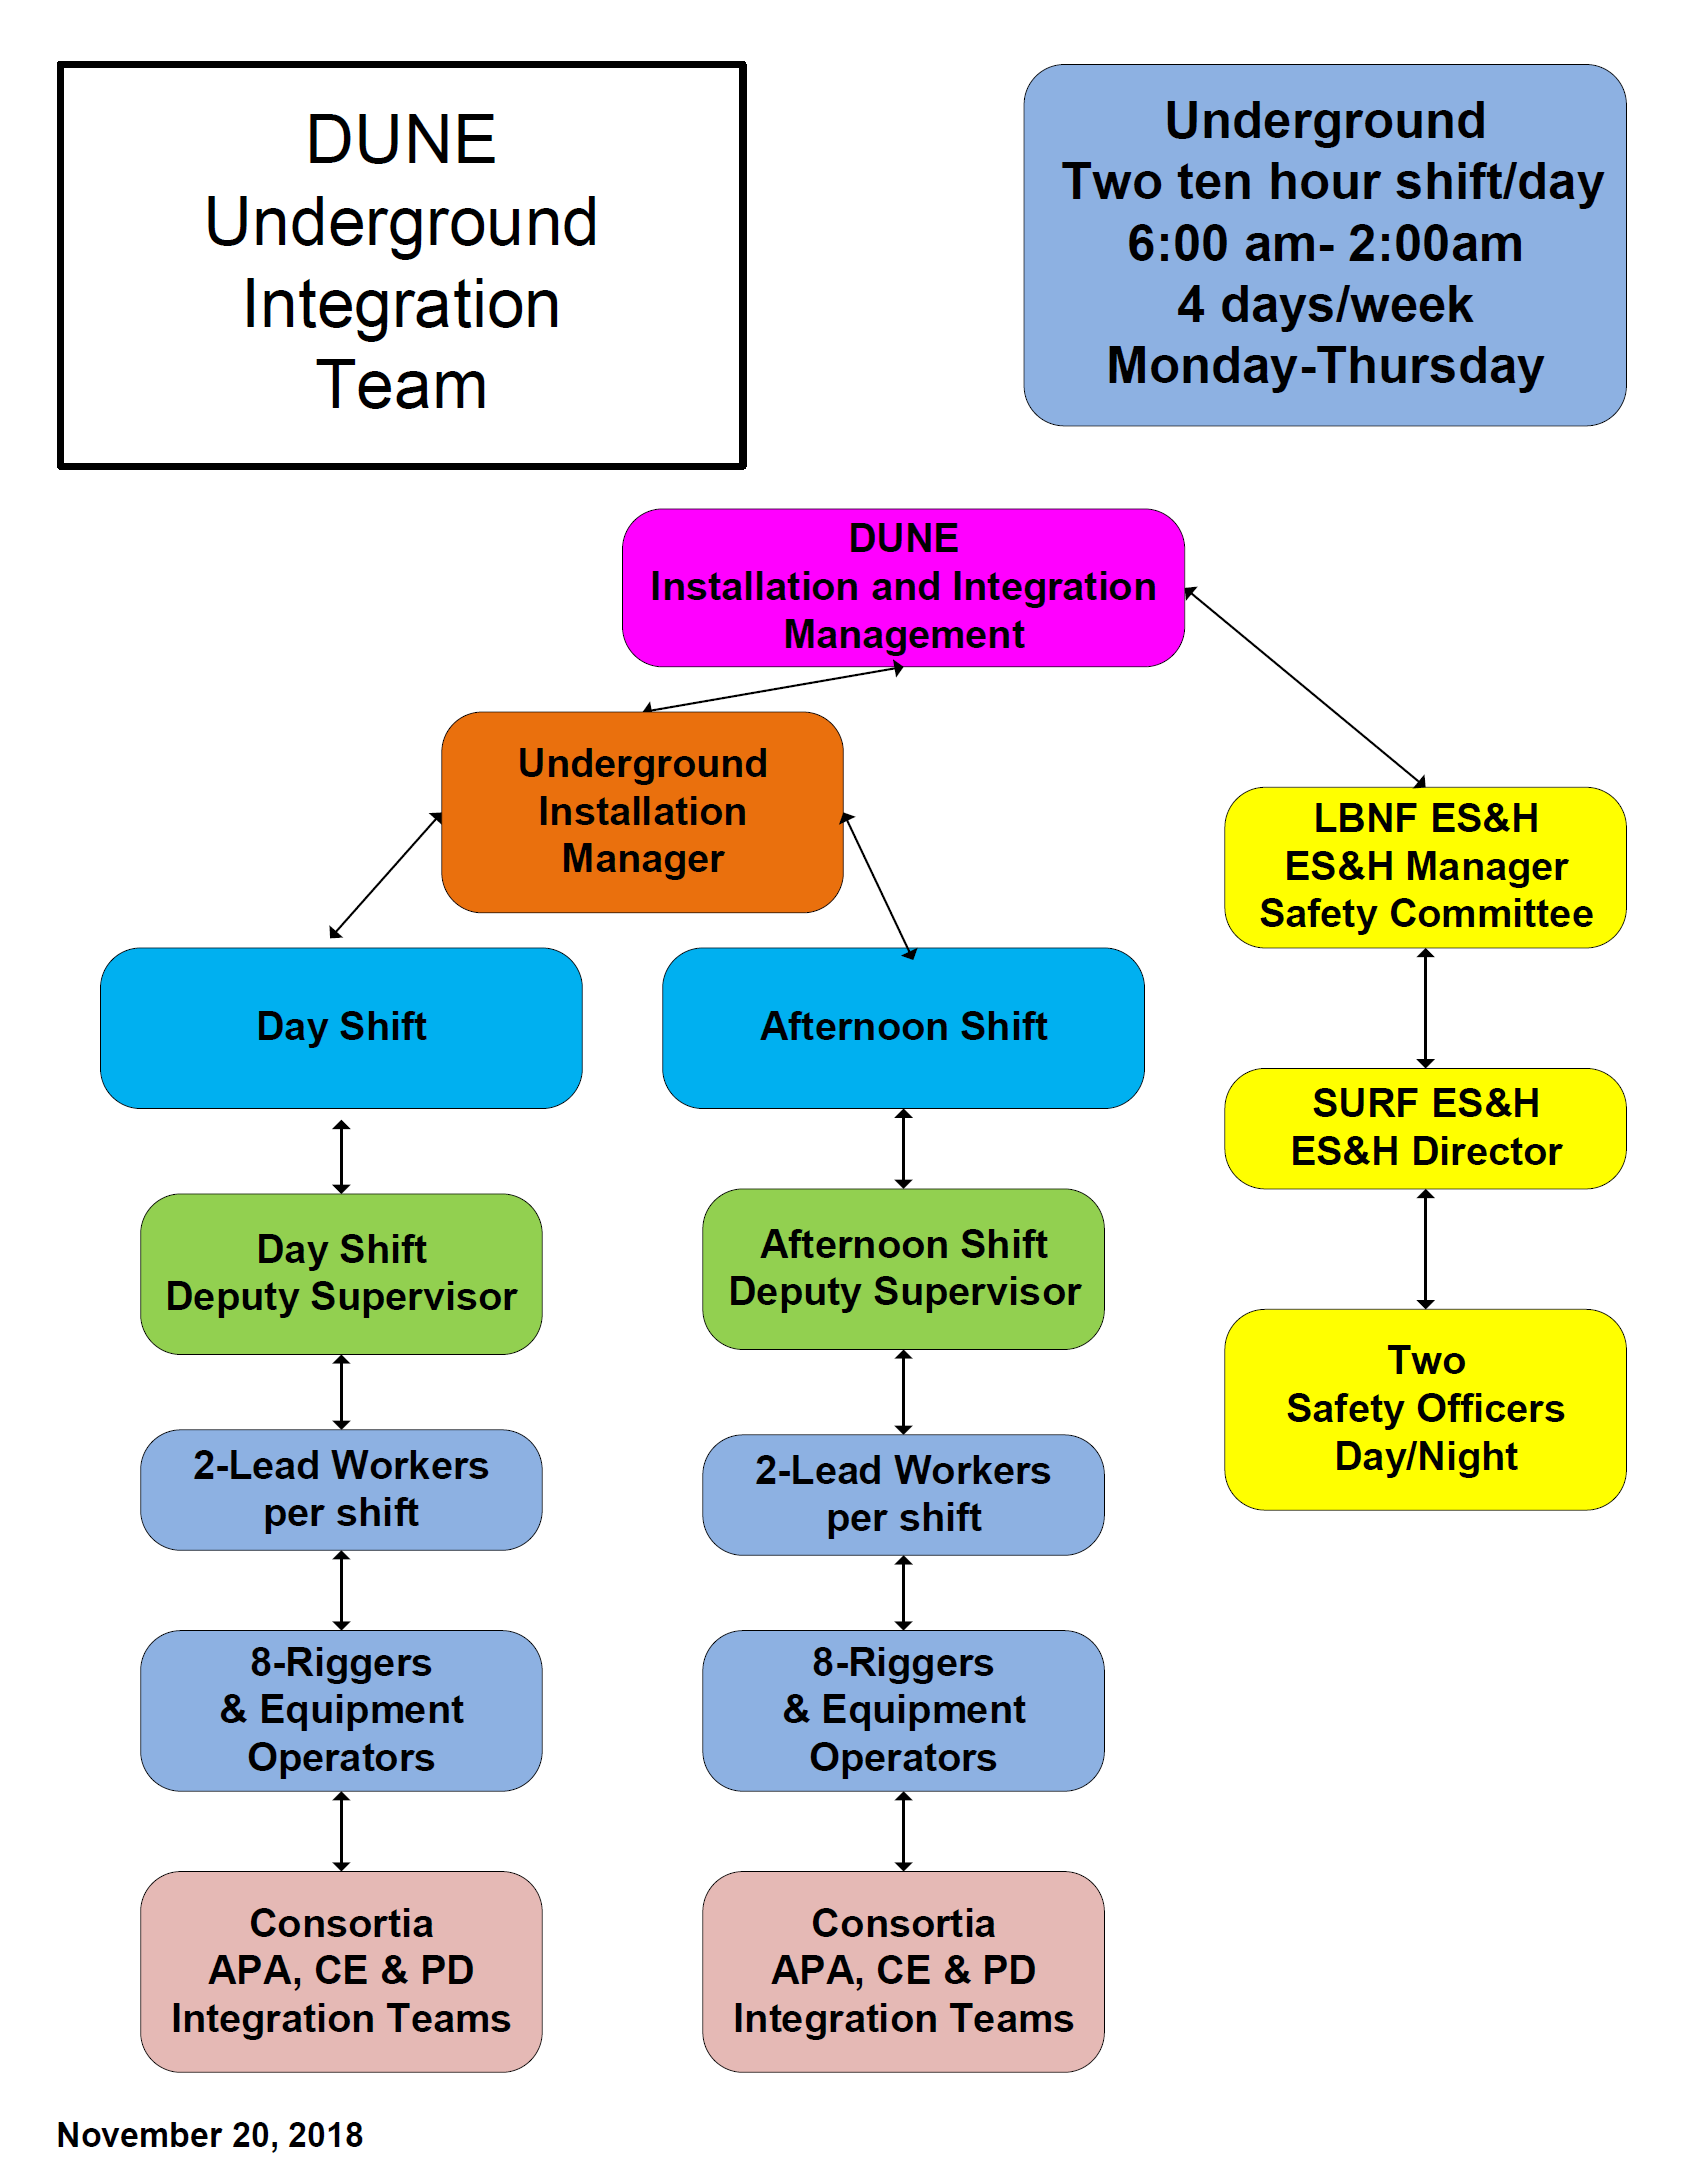
\includegraphics[width=0.85\textwidth]{uit.png}
\end{dunefigure}
and consists of three levels:
\begin{itemize}
  \item Underground Installation Manager --- The UIT manager oversees
    both shifts but also covers for the day or night shift deputy
    manager if needed.  He is the contact person which works directly
    with the Logistic Manager and {surf}/{cmgc} for organization of cage
    trips for materials needed underground.  He attends all high-level
    meetings as required and submits weekly reports.  He schedules and
    organizes the work needed with the Consortia to insure they have
    the rigging crews needed at the appropriate time.
  \item Day/Night Deputy Installation Supervisors --- The deputy
      supervisors are working managers and are trained
      riggers/equipment operators that can fill in as needed.  They
      have been trained in all of the installation procedures and work
      directly with the Consortia to insure that the project remains
      on schedule.  If the lead worker is sick/vacation, they fill in
      this roll. Communication between the deputy supervisors between
      shifts is critical to help a smooth shift change.
  \item Lead Workers --- The lead workers typically are the main
    equipment operators and direct the individual teams typically 2-3
    riggers/equipment operators.  The lead workers are trained in all
    the installation procedures and help the consortia when needed for
    each task.  There are 2 lead workers per shift and would shift as
    needed between the main cavern, materials SAS, cleanroom and
    inside and on top of the cryostat.
  \item Riggers and Equipment Operators --- Riggers and equipment
    operators are trained as both riggers and equipment operators and
    can run the cranes, forklifts and other equipment as needed.  They
    work in minimum of two person teams, more depending on the
    task. Typical APA movement requires a minimum of 3 plus a
    spotter. They are also well training in all the installation
    procedures and can help as needed.
\end{itemize}

\section{Ash River}

The trial assembly work at Ash River has three major phases of DUNE
mechanical tests to confirm designs particularly where things have
been modified from ProtoDUNE.  The NOvA Far Detector Lab is managed by
the University of Minnesota (UMN), which is funded through an
operations grant from Fermilab.  We follow both UMN and Fermilab
safety regulations, whichever is more stringent.  The UMN code
officials approve all building permits, which must include engineered
drawings signed by a Minnesota registered engineer. All hazard
analyses and work procedure documents are approved by a joint safety
committee with members from UMN and Fermilab and may include any
specialist when needed.

There are three main goals for the work at Ash River. Verify that
installation of the DUNE TPC is possible in a safe and efficient
way. Complete a set of procedural documents that will be the basis of
documentation for work underground.  And as a training center for new
hires at {surf} so the procedures are well understood before they happen
underground.

There is a full time staff of five FTEs at Ash River. A manager,
deputy manager and 3 experienced technicians.  One of the technicians
is also our safety officer and is the chairperson of the joint safety
committee.


Phase 0: This work has started now.  A vertical cable test of two
full-scale APA side tubes have been mounted to a column in the
lab. Using a complete cable bundle we will test how well the conduit
system works and what modifications need to be made. We have also
completed a series of different mounting schemes for the ground plane
on the field cage.

Phase 1: We will construct an APA tower using a steel frame large
enough to hold a commercial stair scaffold in the middle as can be
seen in Figure ~\ref{fig:ashriver1}.
\begin{dunefigure}[View of the Ash River Phase 1 assembly.]{fig:ashriver1}
  {Phase 1 Trial Assembly APA Tower at the NOvA Far Detector Lab in Ash River.}
  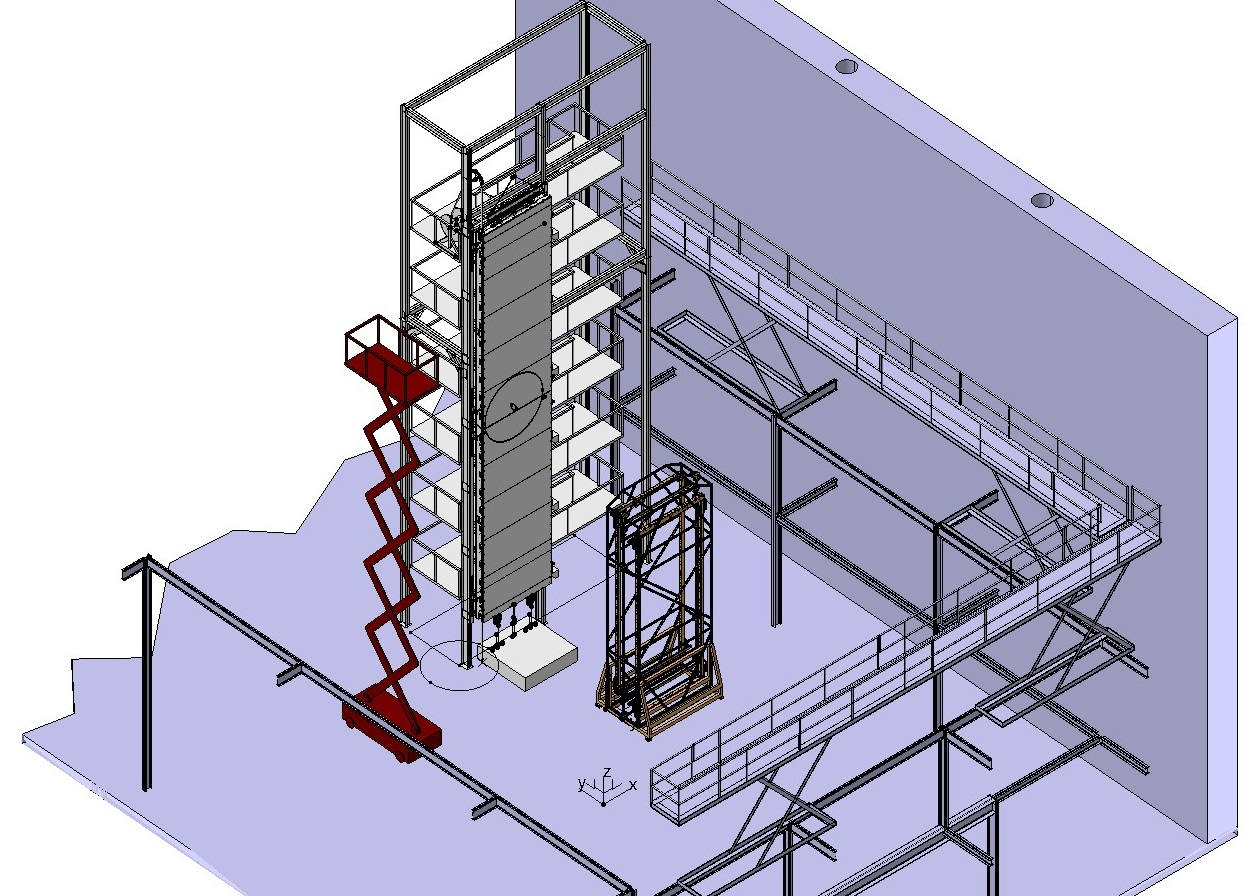
\includegraphics[width=0.85\textwidth]{phase1.jpg}
\end{dunefigure}
This APA tower will be designed so we can
use it for joining the top and bottom APAs together and all the
cabling. Procedures for removing the cable conduits and replacing
failed Photon Detectors will also be developed.

Phase 2: A more complex structure, which mocks up the shuttle
beam/crane in the cleanroom will be needed. A schematic can be seen in
Figure~\ref{fig:ashriver2}.
\begin{dunefigure}[View of the cleanroom for the DUNE-SP detector \#1 showing the shuttle beam system]{fig:ashriver2}
  {View of the cleanroom for the DUNE-SP detector \#1 showing the shuttle beam system}
  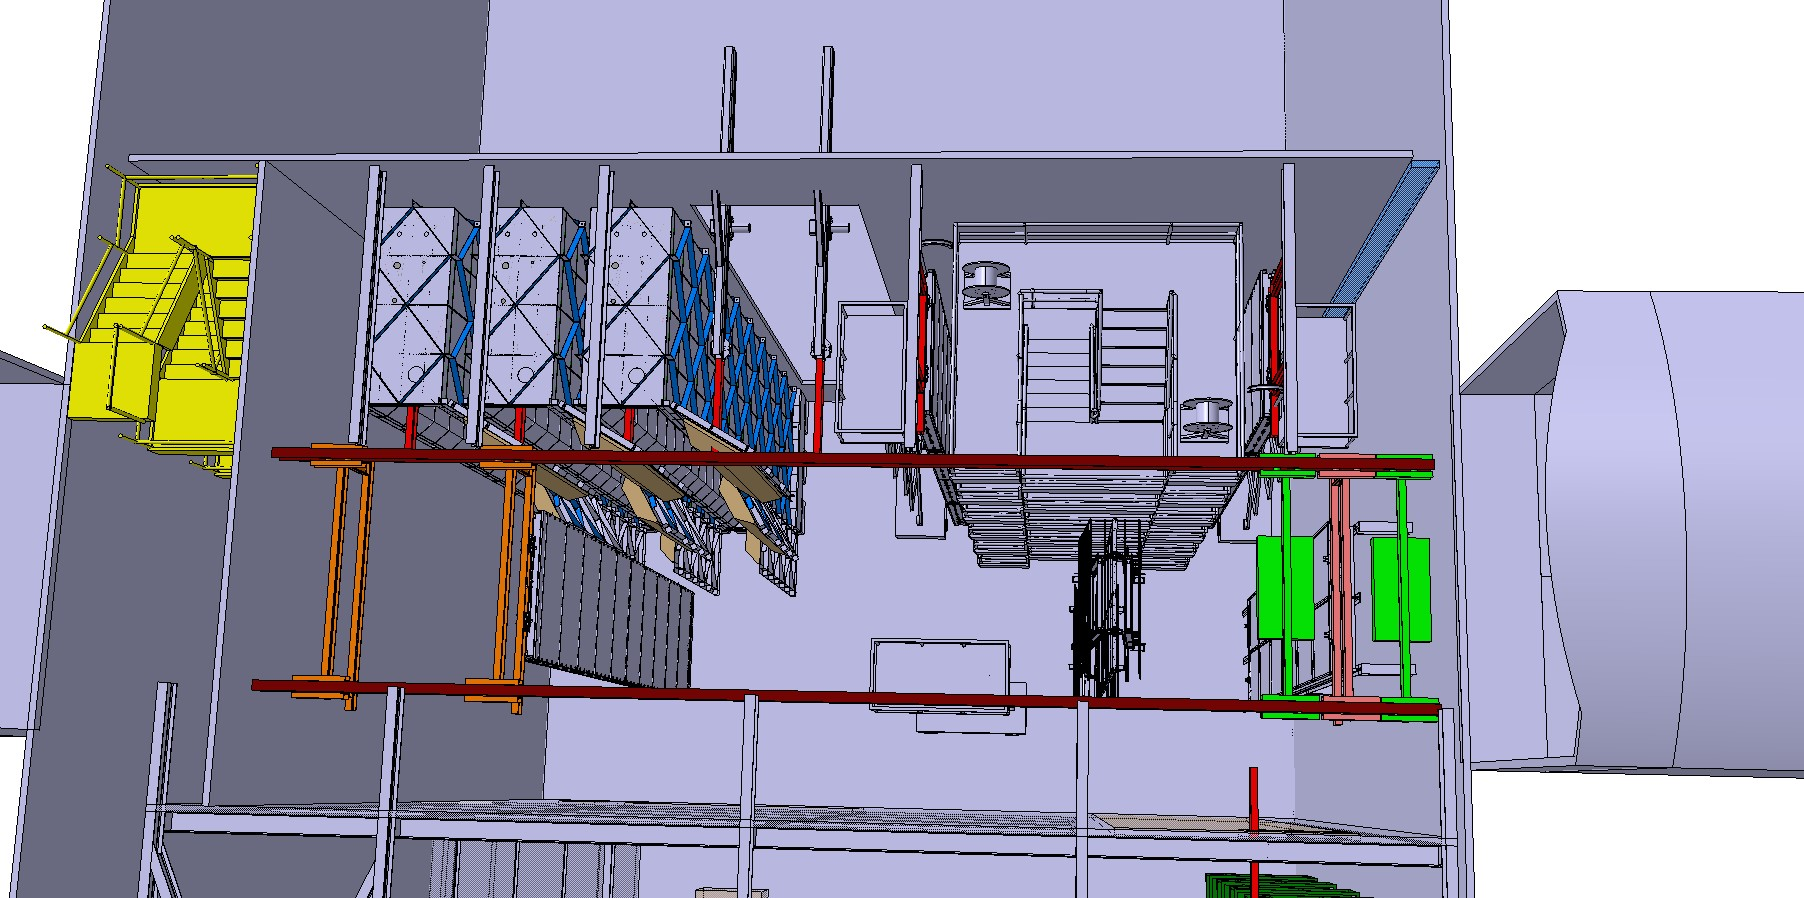
\includegraphics[width=0.85\textwidth]{phase2.jpg}
\end{dunefigure}
This is a very similar to the existing
design of the shuttle beam in the cryostat.  As we proceed with the
phase 1 tests, we will adapt the cleanroom rail system or cryostat
rail system to allow full movement of the APA and CPA pairs. We would
decide how best to allow us to do a full-scale test of the rest of the
installation procedures using this structure including:
\begin{itemize}
 \item Installation of the Detector Support System (DSS)
 \item Transfer of TPC component through the TCO
 \item Moving APA and CPA pairs into ``final'' position and deploying the field cages
 \item Cabling of the APA through the cryostat penetrations
 \item Installation of the end walls
 \item Potentially deployment of the Dual Phase detector
\end{itemize}
